\documentclass[UTF8,a4paper,12pt]{ctexrep}

\usepackage{geometry}
\usepackage{graphicx}
\usepackage{booktabs}
\usepackage{array}
\usepackage[table]{xcolor}
\usepackage{tabularx}
\usepackage{tikz}
\usepackage{float}
\usepackage{hyperref}
\usepackage{enumitem}
\usepackage{caption}
\usetikzlibrary{arrows.meta,positioning,fit}

\geometry{left=2.8cm,right=2.6cm,top=2.8cm,bottom=2.8cm}
\hypersetup{
  colorlinks=true,
  linkcolor=black,
  urlcolor=blue,
  citecolor=black
}
\setlist{nosep}
\renewcommand{\arraystretch}{1.35}
\setlength{\tabcolsep}{7pt}
\definecolor{tablehead}{HTML}{EAF0F7}
\definecolor{tablealt}{HTML}{F7F9FC}
\definecolor{tableline}{HTML}{AEB8C4}
\arrayrulecolor{tableline}
\captionsetup[table]{font=small,labelfont=bf,skip=6pt}
\newcolumntype{L}[1]{>{\raggedright\arraybackslash}m{#1}}
\renewcommand\tabularxcolumn[1]{m{#1}}
\newcolumntype{Y}{>{\raggedright\arraybackslash}X}
\tikzset{
  block/.style={draw=tableline, rounded corners=2pt, fill=tablealt, align=center, minimum height=9mm, font=\small, inner sep=4pt},
  coreblock/.style={draw=tableline, rounded corners=2pt, fill=tablehead, align=center, minimum height=10mm, font=\small\bfseries, inner sep=4pt},
  bus/.style={draw=tableline, fill=white, align=center, minimum height=7mm, font=\small, inner sep=3pt},
  flow/.style={-{Stealth[length=2mm]}, draw=tableline, line width=0.45pt}
}

\title{基于 ROSbot XL 的室内自主移动机器人嵌入式系统解决方案分析}
\author{}
\date{}

\begin{document}

\maketitle

\begin{abstract}
ROSbot XL 是面向室内移动机器人教学、研发与原型验证的自主移动机器人平台。根据 Husarion 官方公开资料，该平台支持 ROS 2，可选配 Raspberry Pi、NVIDIA Jetson 或 Intel NUC 等上位计算平台，底层控制板包含 STM32F4 微控制器，并通过 Ethernet 与上位计算平台通信。机器人本体集成四个直流电机及编码器、IMU、电源管理板、电池、USB Hub、RGB LED 和扬声器等部件。本文从需求分析、总体结构、基本构件和硬件系统设计四个方面，对 ROSbot XL 的嵌入式系统解决方案进行分析。对于官方资料未公开的具体芯片型号和内部实现细节，不作确定性描述，仅从嵌入式系统工程设计角度给出可理解为、可分析为或工程上通常可采用的实现方式。
\end{abstract}

\tableofcontents

\chapter{项目背景与产品概述}

\section{研究对象与分析范围}

室内自主移动机器人是典型的嵌入式系统综合应用对象，其系统形态同时包含嵌入式计算、实时控制、传感器采集、执行器驱动、通信互联、电源管理和机器人软件框架。ROSbot XL 作为室内自主移动机器人平台，能够承载定位、建图、导航、避障、底盘运动控制以及人机交互等功能，因此适合作为嵌入式系统解决方案分析对象。

分析范围以 ROSbot XL 公开资料中能够确认的系统构成为基础，重点讨论其嵌入式系统架构，而不对官方没有公开的具体芯片型号、PCB 级电路细节或闭源固件实现作确定性推断。根据现有资料，ROSbot XL 的关键公开信息包括：其定位为室内自主移动机器人平台；支持 ROS 2；可选上位计算平台包括 Raspberry Pi、NVIDIA Jetson 与 Intel NUC；底层控制板包含 STM32F4 微控制器；上位计算平台与控制板之间通过 Ethernet 通信；机器人包含四个直流电机和编码器，并集成 IMU、电源管理板、电池、USB Hub、RGB LED 与扬声器等部件。

从嵌入式系统角度看，ROSbot XL 并不是单一处理器系统，而是由上位计算平台、底层实时控制板、传感器、执行器、电源系统和通信网络共同构成的分布式嵌入式系统。其中，上位计算平台承担计算密集型任务和 ROS 2 节点运行；底层控制板承担实时性更强的底盘控制、编码器采集、执行器驱动接口和部分状态监测任务；传感器和执行器构成机器人与物理环境交互的前端。

\section{产品定位与嵌入式属性}

ROSbot XL 的产品定位可理解为面向室内环境的移动机器人开发平台。与纯软件仿真平台不同，ROSbot XL 需要在真实物理环境中完成感知、决策和运动控制，因而其嵌入式系统必须同时满足计算性能、实时控制、通信可靠性、能量约束和机械运动安全等要求。

从系统功能划分看，该机器人具有明显的层次化嵌入式结构。上位计算平台运行 Linux 和 ROS 2 相关软件，面向应用层算法和任务编排；底层 STM32F4 控制板属于典型微控制器子系统，面向电机控制、编码器反馈、低层接口和实时响应。两者之间通过 Ethernet 交换控制命令与状态数据，使系统可以在较高层保持软件生态开放性，同时在底层保留较稳定的实时控制能力。

这种结构体现了现代机器人嵌入式系统的常见设计思路：将高层算法和低层控制分离，通过明确的通信接口连接。工程上通常可采用这种分层方式降低系统耦合度，使导航、SLAM 和任务控制软件能够在上位计算平台中迭代，而电机闭环控制、传感器底层采样和安全保护逻辑则保持在实时控制单元中运行。

\section{资料来源与分析边界}

Husarion 官方手册公开说明了 ROSbot XL 的软件支持、计算平台选项、控制板、通信方式和若干硬件构件。处理器分析部分还参考了 STM32F405/407 数据手册和 BCM2711 ARM Peripherals 文档，用于说明 STM32F4 系列微控制器以及 Raspberry Pi 4B 所用 BCM2711 平台的典型处理器与外设特征。对于公开资料中未明确给出的 ROSbot XL 实际处理器具体子型号、外设芯片型号、驱动器型号、传感器精确型号和电路连接细节，本报告仅在系统层面进行分析，不作超出公开信息的确定性描述。

因此，在描述嵌入式处理器、传感器接口和执行器接口时，需区分事实性信息与工程分析性判断。前者是公开资料中能够确认的内容，例如“底层控制板包含 STM32F4 微控制器”“SBC 与控制板之间通过 Ethernet 通信”；后者是在嵌入式系统设计规律基础上给出的合理解释，例如“可理解为上位计算与实时控制的分层架构”“工程上通常可采用 PWM 驱动直流电机并通过编码器反馈形成闭环控制”。这种区分有助于避免将工程推断误写为产品规格。

\chapter{需求分析}

\section{功能需求}

ROSbot XL 的功能需求应围绕室内自主移动机器人这一嵌入式系统对象展开。机器人需要完成的不只是软件层面的路径规划，还包括传感器采集、实时运动控制、执行器驱动、能量供给和通信协同等嵌入式任务。

第一，机器人需要具备移动底盘控制能力。根据公开资料，ROSbot XL 包含四个直流电机和编码器。由此可分析为，系统需要接收上位计算平台给出的速度或运动控制命令，并在底层控制板上转换为对四个电机的驱动输出。同时，编码器反馈需要用于估计轮速、里程计和底盘运动状态，为闭环控制和导航算法提供基础数据。

第二，机器人需要具备环境感知与状态感知能力。公开资料中确认其包含 IMU，并可作为 ROS 2 移动机器人平台使用。IMU 可用于角速度、加速度等运动状态测量；在室内自主导航场景中，工程上通常还会结合 LiDAR、深度相机或其他外部传感器进行障碍物检测、建图和定位。若具体传感器型号未由官方资料明确给出，则仅将其作为可扩展感知单元分析，而不指定具体芯片或模块型号。

第三，机器人需要支持自主导航相关功能。作为室内自主移动机器人平台，其上位计算平台需要运行 ROS 2 节点，完成传感器数据接收、坐标变换、地图构建、定位、路径规划和速度命令输出等任务。从嵌入式系统角度看，这些功能依赖上位处理器的通用计算能力、操作系统调度能力和外设通信能力。

第四，机器人需要支持底层执行和人机反馈功能。公开资料列出了 RGB LED 和扬声器等部件。它们可理解为嵌入式系统中的状态显示和提示输出装置，用于表达运行模式、故障状态、电量状态或交互提示。底层控制板或上位计算平台可通过相应接口对其进行控制。

第五，机器人需要具备电源管理能力。公开资料显示系统包含电源管理板和电池。对于移动机器人而言，电源子系统不仅提供供电，还需要支持电池状态监测、供电分配和欠压保护等功能。工程上通常可采用电源管理板将电池电压转换为不同负载所需电压轨，并向控制系统提供电量、充电或保护状态信息。

\section{非功能需求}

非功能需求决定嵌入式系统能否稳定、可靠地在真实环境中运行。对于 ROSbot XL 这类移动机器人，非功能需求至少包括实时性、可靠性、可扩展性、安全性、功耗约束和可维护性。

实时性是底层控制子系统的核心要求。电机控制、编码器采样和底盘状态更新需要以稳定周期执行，否则容易导致速度响应滞后、里程计误差增大或运动不平稳。采用 STM32F4 微控制器承担底层控制任务，可理解为通过微控制器的定时器、中断和外设接口实现确定性更强的实时任务执行，而将非实时或弱实时的高层算法交给上位计算平台处理。

可靠性要求系统在通信抖动、传感器异常或电源波动等情况下仍能保持可控状态。SBC 与控制板之间通过 Ethernet 通信，这有利于提供较高带宽和较规范的网络通信接口；但机器人底层仍需要具备在通信中断或命令超时情况下进入安全状态的能力。工程上通常可采用看门狗、通信超时检测、急停输入、速度限幅和低电压保护等机制增强可靠性。

可扩展性体现在硬件外设和软件生态两个层面。硬件上，USB Hub、Ethernet 和上位计算平台为扩展 LiDAR、深度相机、调试设备或其他传感器提供了基础条件。软件上，ROS 2 的节点化和消息通信机制便于扩展感知、导航和任务应用。对嵌入式系统而言，这种可扩展性需要建立在清晰的接口边界和稳定的数据通路之上。

安全性包括电气安全、运动安全和软件安全。移动机器人在室内运行时需要避免失控运动、碰撞和电池异常。底层控制系统应对电机输出、电源状态和通信状态进行约束；上位系统应对导航目标、速度命令和障碍物信息进行校验。若官方资料未公开具体安全电路，则可从系统设计要求层面分析其必要性。

功耗与热设计也是移动嵌入式系统的重要约束。上位计算平台、电机、电源管理板和外设传感器均消耗电池能量。可选计算平台从 Raspberry Pi 到 NVIDIA Jetson 或 Intel NUC，其性能、功耗和散热特性差异较大。系统设计需要在算法性能、续航时间和热稳定性之间取得平衡。

\section{需求到嵌入式系统指标的映射}

将上述需求映射到嵌入式系统指标，可形成表 \ref{tab:req-map} 所示的分析关系。该映射不依赖具体未公开芯片型号，而是从系统构件职责出发说明需求如何落实到嵌入式设计中。

\begin{table}[H]
  \centering
  \caption{需求与嵌入式系统指标映射}
  \label{tab:req-map}
  \small
  \begin{tabularx}{\textwidth}{L{3.0cm}L{4.0cm}Y}
    \toprule
    \rowcolor{tablehead}
    \textbf{需求类别} & \textbf{嵌入式指标} & \textbf{设计含义} \\
    \midrule
    \rowcolors{2}{tablealt}{white}
    底盘运动控制 & 控制周期、编码器采样频率、输出稳定性 & 由底层控制板承担周期性控制任务，保证电机输出与反馈采集的实时性。 \\
    自主导航 & 计算性能、传感器吞吐、操作系统支持 & 由 SBC 运行 Linux 和 ROS 2，处理地图、定位、规划和速度命令生成。 \\
    状态感知 & 传感器接口、时间同步、数据质量 & IMU、编码器及可扩展感知设备需要通过稳定接口向控制与导航模块提供数据。 \\
    通信协同 & Ethernet 带宽、延迟、协议稳定性 & SBC 与 STM32F4 控制板之间通过 Ethernet 交换控制命令与状态信息。 \\
    移动供电 & 电压转换、电量监测、保护机制 & 电源管理板和电池为处理器、传感器和执行器提供分层供电。 \\
    可维护扩展 & 模块化接口、ROS 2 软件生态、调试接口 & 通过标准化软硬件接口降低二次开发难度。 \\
    \bottomrule
    \rowcolors{2}{}{}
  \end{tabularx}
\end{table}

\chapter{系统总体结构}

\section{系统总体架构}

ROSbot XL 的总体结构可理解为“上位计算平台 + 底层实时控制板 + 传感器与执行器 + 电源管理”的嵌入式机器人架构。该结构将机器人系统中的任务按照计算复杂度、实时性和接口位置进行划分，使不同子系统承担不同职责。

上位计算平台通常采用 SBC（Single Board Computer，即单板计算机）形态，官方资料给出的可选平台包括 Raspberry Pi、NVIDIA Jetson 和 Intel NUC。由于这些平台的具体型号可按配置变化，分析中不指定具体芯片型号。SBC 主要面向 Linux、ROS 2 和机器人应用软件，承担计算量较大的任务，例如感知数据处理、SLAM、定位、路径规划、任务调度和用户交互。

底层实时控制板包含 STM32F4 微控制器。STM32F4 属于 ARM Cortex-M 系列微控制器产品族，适合承担电机控制、编码器采集、周期性任务调度和底层外设接口管理等任务。相较于运行通用操作系统的 SBC，微控制器通常具有更强的实时可预测性和更直接的外设控制能力。

传感器与执行器构成机器人嵌入式系统的物理输入输出层。编码器和 IMU 提供运动状态反馈；可扩展的 LiDAR、深度相机等传感器可为环境感知提供数据；四个直流电机则将控制命令转换为机器人运动。RGB LED 和扬声器属于低速输出外设，可用于状态反馈和提示。

电源系统由电池和电源管理板构成，为不同电压、不同功耗等级的负载供电。移动机器人系统中的电源管理不仅影响续航能力，也直接影响控制稳定性和硬件可靠性。

\section{软硬件协同结构}

从软硬件协同角度看，ROSbot XL 可分析为分层控制系统。高层软件运行在 SBC 上，使用 ROS 2 提供的通信、节点管理和机器人算法生态；低层固件运行在 STM32F4 控制板上，负责将上位速度命令转化为执行器控制，并将编码器、IMU 或底盘状态反馈给上位系统。

这种协同结构的核心是明确高层与低层之间的数据边界。SBC 不直接承担每一个电机 PWM 输出或编码器边沿捕获，而是通过 Ethernet 与控制板交换抽象程度更高的数据，例如目标速度、底盘状态、里程计相关数据或诊断信息。底层控制板则不承担复杂地图计算，而专注于实时控制和硬件接口。这样可以降低系统复杂度，并提高不同层级的可替换性。

在嵌入式系统中，软硬件协同还体现为数据时序匹配。传感器采样、控制计算和执行器输出需要形成稳定闭环；上位导航算法的更新频率通常低于底层电机控制频率。因此，工程上通常可采用多周期协同方式：底层控制以较短周期执行速度闭环，上位规划以较长周期输出速度指令，二者通过通信协议进行同步。

\section{硬件结构概述}

ROSbot XL 的硬件结构可按功能划分为计算控制、感知、执行、电源和通信五类模块。

计算控制模块包括 SBC 和 STM32F4 控制板。SBC 作为高层嵌入式计算节点，负责运行操作系统和机器人软件；STM32F4 控制板作为底层微控制器节点，负责实时控制和硬件接口。二者通过 Ethernet 相连，形成分布式控制架构。

感知模块包括编码器、IMU 以及可扩展的外部感知设备。编码器通常与电机或轮系连接，用于测量轮速和位移增量；IMU 用于测量惯性运动信息；外部感知设备可根据应用需求接入，用于环境建图、障碍物检测或视觉感知。由于具体外部传感器型号未在公开资料中明确，相关分析仅讨论其系统接口角色。

执行模块包括四个直流电机、RGB LED 和扬声器等。直流电机是底盘运动执行器，通常需要驱动电路完成电流放大和方向控制；RGB LED 与扬声器属于状态提示类执行器，对实时性要求相对较低，但对用户理解机器人状态具有重要作用。

电源模块包括电池和电源管理板。电池提供移动能源，电源管理板完成电源分配、转换和保护。对于含有电机和高性能计算平台的机器人，电源系统需要同时支持大电流瞬态负载和稳定数字电源供应。

通信模块包括 Ethernet、USB Hub 及其他可能的板级外设接口。Ethernet 用于 SBC 与底层控制板之间通信；USB Hub 可为传感器、调试设备或其他外设提供扩展连接。工程上通常还会在控制板内部使用 UART、I2C、SPI、PWM、ADC、GPIO、定时器输入捕获等接口连接不同外设，但具体接口分配需以官方硬件资料为准。

\section{软件结构概述}

虽然本报告前四章以需求和硬件系统为主，但 ROSbot XL 的软件结构仍是理解嵌入式系统总体架构的必要组成。公开资料确认 ROSbot XL 支持 ROS 2，因此其上位软件可理解为围绕 ROS 2 节点、话题、服务、参数和启动文件组织。

上位软件层通常包括设备驱动与接口节点、状态估计与里程计节点、SLAM 或定位节点、路径规划与控制节点以及任务应用节点。底层固件则通常包括通信协议解析、传感器采样、电机控制、状态反馈和故障处理等模块。二者通过 Ethernet 进行数据交互。

这种软件结构体现了嵌入式系统中“实时控制固件 + 通用操作系统应用”的组合形态。其优势在于既能够利用 ROS 2 的生态完成复杂算法开发，又能够通过微控制器固件保持底层控制的实时性和稳定性。

\section{关键构件说明}

根据作业要求，除系统总体结构外，还需要说明嵌入式系统中的基本构件。ROSbot XL 的关键构件可按“计算控制、感知、执行、电源、通信、软件”六类理解。各构件并非孤立存在，而是通过接口和软件协议共同构成闭环控制系统：传感器提供状态输入，处理器完成计算和控制决策，执行器作用于物理环境，电源模块维持移动运行，通信模块连接不同处理单元，软件则负责调度和组织功能。

\begin{table}[H]
  \centering
  \caption{ROSbot XL 关键构件及嵌入式系统职责}
  \label{tab:key-components}
  \small
  \begin{tabularx}{\textwidth}{L{3.0cm}L{3.6cm}Y}
    \toprule
    \rowcolor{tablehead}
    \textbf{构件类别} & \textbf{代表构件} & \textbf{嵌入式系统职责} \\
    \midrule
    \rowcolors{2}{tablealt}{white}
    上位计算构件 & Raspberry Pi、NVIDIA Jetson、Intel NUC 等 SBC & 运行 Linux 和 ROS 2，承担 SLAM、导航、路径规划、外设驱动和任务管理等高层计算。 \\
    底层控制构件 & STM32F4 控制板 & 负责电机控制、编码器采集、底层传感器读取、状态反馈和安全保护。 \\
    感知构件 & 编码器、IMU、可扩展 LiDAR 或深度相机 & 获取轮速、姿态、环境和障碍物信息，为定位、建图和闭环控制提供输入。 \\
    执行构件 & 四个直流电机、RGB LED、扬声器 & 将控制信号转换为底盘运动和人机提示输出。 \\
    电源构件 & 电池、电源管理板 & 提供移动供电、电压转换、电源分配和电量或故障状态反馈。 \\
    通信与扩展构件 & Ethernet、USB Hub、GPIO、I2C、SPI、UART 等 & 连接上位计算平台、底层控制板、传感器和扩展外设，形成系统数据通路。 \\
    软件构件 & ROS 2 节点、Linux 驱动、底层固件 & 组织传感器数据、控制命令、状态反馈和应用任务，实现软硬件协同。 \\
    \bottomrule
    \rowcolors{2}{}{}
  \end{tabularx}
\end{table}

\chapter{硬件系统设计}

\section{硬件系统框图}

图 \ref{fig:hardware-block} 给出了 ROSbot XL 硬件系统的结构框图。该图从嵌入式系统角度展示了上位计算平台、STM32F4 控制板、传感器、执行器、电源管理和通信接口之间的关系。需要说明的是，框图用于描述系统级连接和功能分工；对于官方资料未公开的具体芯片型号、驱动芯片型号和 PCB 级细节，不作展开。

\begin{figure}[H]
  \centering
  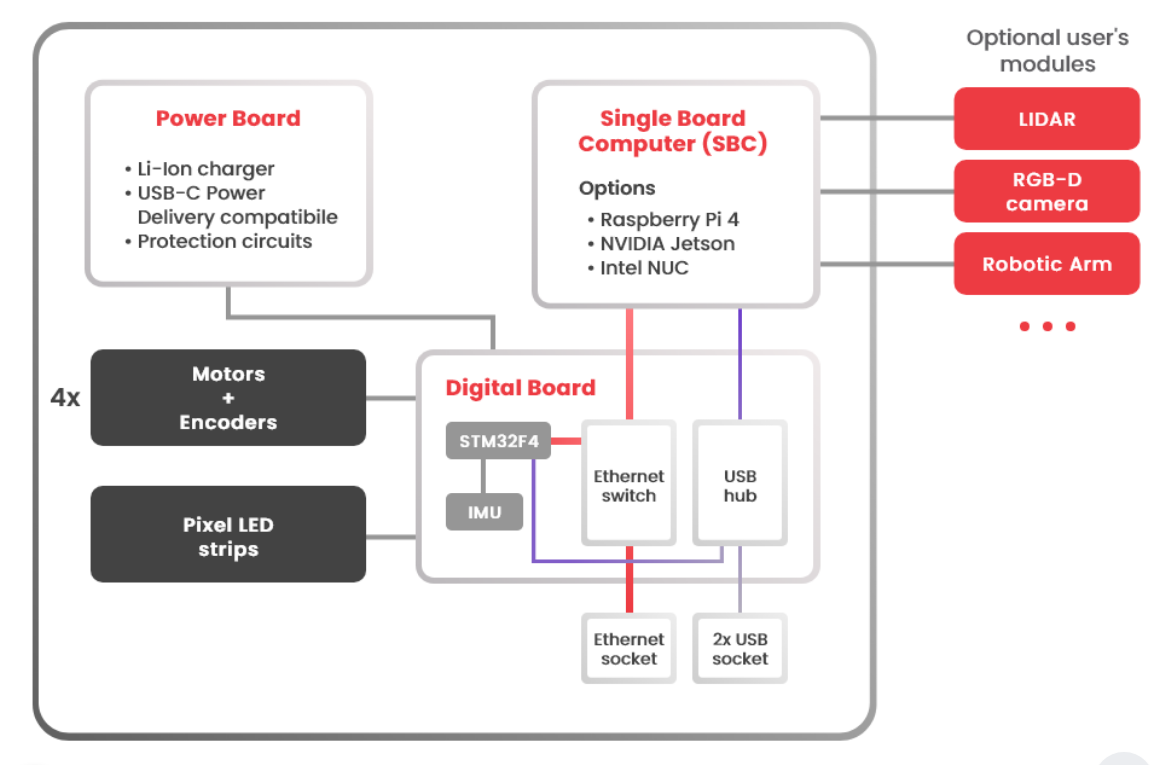
\includegraphics[width=0.95\textwidth]{assets/rosbot_xl_hardware_block.png}
  \caption{ROSbot XL 硬件系统框图}
  \label{fig:hardware-block}
\end{figure}

从框图可见，ROSbot XL 的硬件系统可理解为以 SBC 和 STM32F4 控制板为核心的双处理器结构。SBC 负责高层计算任务，STM32F4 控制板负责底层实时控制任务；传感器、执行器和电源管理模块围绕二者形成机器人完整的嵌入式硬件平台。

\section{上位计算平台 SBC}

ROSbot XL 官方资料列出的可选上位计算平台包括 Raspberry Pi、NVIDIA Jetson 和 Intel NUC。由于这些平台均包含多个具体产品型号，且公开资料未限定唯一型号，系统分析中将其统称为 SBC 或上位计算平台，而不引入具体处理器芯片型号。

SBC 在嵌入式系统中的主要作用是提供运行 Linux 和 ROS 2 的计算环境。与微控制器相比，SBC 通常具有更高的主频、更大的内存、更完整的操作系统支持以及更丰富的网络和 USB 外设能力，适合运行 SLAM、导航、视觉处理、任务管理和远程调试等软件。

从硬件接口角度看，SBC 至少需要与底层控制板通过 Ethernet 通信，并通过 USB Hub 或自身外设接口连接传感器、调试设备和扩展模块。不同 SBC 的选择会影响功耗、散热、计算能力和接口数量，但不改变系统的基本分层控制思想。关于 SBC 处理器结构、内核类型和内部接口的详细分析，将在第 5 章展开。

\section{底层实时控制板 STM32F4}

底层控制板包含 STM32F4 微控制器，这是 ROSbot XL 嵌入式硬件系统中的实时控制核心。由于公开资料仅说明为 STM32F4，分析中不指定具体 STM32F4 子型号。

从系统职责看，STM32F4 控制板可分析为底盘控制和外设实时接口中心。它需要接收来自 SBC 的控制命令，并完成电机驱动控制、编码器采集、部分传感器数据读取、状态打包与反馈等任务。该控制板在硬件系统中的核心价值是提供比通用操作系统更稳定的底层实时控制能力。

在四轮直流电机系统中，底层控制板通常需要管理多个电机通道，并结合编码器反馈形成底盘运动控制闭环。STM32F4 的内部组件、Cortex-M4 内核、指令集架构以及与底层任务的对应关系，将在第 5 章进行专门分析。

\section{传感器系统}

ROSbot XL 公开资料中确认包含编码器和 IMU。编码器直接服务于底盘运动控制，是移动机器人里程计估计的重要来源。IMU 则提供角速度和加速度等惯性信息，可辅助姿态估计、运动状态判断和导航算法。

编码器与电机形成紧密耦合的反馈链路。对于嵌入式控制系统而言，编码器信号需要以较高可靠性输入到底层控制板。工程上通常可采用定时器编码器模式、输入捕获或外部中断方式读取编码器脉冲，并根据单位时间内的脉冲数计算轮速。编码器数据一方面用于底层速度闭环控制，另一方面可经由控制板上传给 SBC，用于里程计和定位。

IMU 的接口取决于具体模块实现。由于公开资料未说明具体 IMU 型号，分析中不指定其芯片型号或总线协议。工程上通常可采用 I2C、SPI 或 UART 等接口连接 IMU，并通过周期采样或中断方式获取数据。IMU 数据在机器人系统中通常需要与编码器里程计、外部定位或 SLAM 结果进行融合，以提高状态估计稳定性。

对于 LiDAR、深度相机等环境感知设备，可将其作为室内自主导航中工程上通常可采用的扩展传感器讨论。此类设备一般与 SBC 直接连接，因为其数据量较大，并且需要 ROS 2 驱动节点进行数据处理。USB、Ethernet 或专用相机接口都可能用于连接外部感知设备，具体方式取决于实际配置。

\section{执行器系统}

ROSbot XL 包含四个直流电机和编码器。直流电机是底盘运动的主要执行器，需要由控制板通过电机驱动器进行控制。由于公开资料未给出驱动器具体型号，相关内容仅从嵌入式系统接口角度进行分析。

直流电机控制通常包括转速控制、方向控制和制动控制等功能。工程上通常可采用 PWM 调制方式改变电机平均电压或驱动占空比，通过方向控制信号改变转向，并结合编码器反馈形成闭环。对于四电机平台，控制板需要保证各通道控制周期一致，并处理电机之间的速度匹配问题。

RGB LED 和扬声器属于提示类执行器。RGB LED 可用于显示系统状态、运行模式或异常报警；扬声器可用于声音提示。它们的控制实时性要求通常低于电机，但在机器人可维护性和人机交互中具有实际价值。工程上通常可通过 GPIO、PWM 或串行接口控制此类外设。

\section{电源管理系统}

移动机器人依赖电池供电，ROSbot XL 公开资料中也列出了电池和电源管理板。电源管理系统是嵌入式硬件可靠运行的基础，需要为 SBC、控制板、传感器、USB 外设和电机驱动提供合适的电源。

从负载特性看，电机属于大电流、强动态负载；SBC 和控制板属于数字计算负载；传感器和 USB 外设则可能对电源纹波和电压稳定性较敏感。因此，电源管理板可理解为系统中的电源分配与转换中心。工程上通常可采用多路 DC-DC 转换、保险或过流保护、欠压检测、电池电量监测和电源开关控制等设计，但具体实现需以官方硬件资料为准。

电源状态还应进入控制系统的监测范围。例如，当电池电压过低时，系统应限制电机输出或进入保护状态；当外设供电异常时，系统应向上位软件报告诊断信息。这些功能体现了嵌入式系统中硬件保护与软件策略的协同。

\section{通信接口系统}

ROSbot XL 官方资料明确说明 SBC 与控制板之间通过 Ethernet 通信。Ethernet 在机器人系统中具有带宽较高、协议成熟、调试方便和扩展性较好的优点，适合作为上位计算平台与底层控制板之间的主通信链路。

在该链路中，SBC 可向控制板发送速度命令、模式切换命令或配置参数；控制板可向 SBC 返回编码器数据、底盘状态、电源状态和诊断信息。通信协议需要考虑数据格式、刷新周期、超时处理和错误检测。工程上通常可采用周期性状态报文和命令报文配合的方式，使高层导航与底层控制保持同步。

除 Ethernet 外，USB Hub 也是 ROSbot XL 的重要扩展部件。USB Hub 可用于连接外部传感器、输入设备、调试设备或其他机器人外设。对于嵌入式系统而言，USB 扩展能力有助于提高平台通用性，但也要求系统关注带宽分配、供电能力和设备枚举稳定性。

在控制板内部，STM32F4 与电机驱动、编码器、IMU、LED、扬声器和电源管理板之间还可能存在多种板级接口。工程上通常可采用 GPIO、PWM、ADC、I2C、SPI、UART、定时器输入捕获等外设资源完成连接。由于具体连接未由公开资料确认，相关内容仅从接口类型和系统职责角度进行分析。

\chapter{嵌入式处理器分析}

\section{处理器总体架构}

ROSbot XL 的嵌入式处理系统可理解为“上位计算平台 + 底层实时控制器”的双处理器协同架构。系统中主要涉及两类嵌入式处理器：一类是作为上位计算平台的 SBC（Single Board Computer，单板计算机），另一类是底层控制板上的 STM32F4 微控制器。

其中，SBC 负责运行 Linux 操作系统和 ROS 2 机器人软件框架，主要承担导航、建图、路径规划、任务调度、远程通信等高层计算任务；STM32F4 微控制器负责底层实时控制，主要承担电机控制、编码器采集、IMU 数据读取、底层外设管理和安全监测等任务。这种双处理器架构将复杂计算任务与实时控制任务分离，使系统既具备较强的高层计算能力，又能保证底层运动控制的实时性和可靠性。

整体处理器分工如表 \ref{tab:processor-division} 所示。

\begin{table}[H]
  \centering
  \caption{ROSbot XL 处理器分工}
  \label{tab:processor-division}
  \small
  \begin{tabularx}{\textwidth}{L{3.4cm}Y L{3.2cm}}
    \toprule
    \rowcolor{tablehead}
    \textbf{处理器模块} & \textbf{主要任务} & \textbf{运行环境} \\
    \midrule
    \rowcolors{2}{tablealt}{white}
    SBC 上位计算平台 & Linux、ROS 2、SLAM、导航、路径规划、任务调度、网络通信 & Linux 与 ROS 2 \\
    STM32F4 控制板 & 电机控制、编码器采集、IMU 读取、外设控制、安全监测 & 裸机程序或 RTOS 固件 \\
    \bottomrule
    \rowcolors{2}{}{}
  \end{tabularx}
\end{table}

从系统功能角度看，SBC 可理解为机器人系统中的高层决策与计算中心，负责判断机器人应如何运动；STM32F4 可理解为底层执行与状态反馈中心，负责把高层指令转换为具体的电机控制，并将底盘状态返回上位计算平台。

\section{SBC 上位计算平台分析}

\subsection{SBC 的系统作用}

在 ROSbot XL 中，SBC（Single Board Computer，即单板计算机）是机器人系统的上位计算平台，主要负责运行操作系统和机器人应用软件。与底层 MCU 相比，SBC 的计算能力更强，能够运行 Linux、ROS 2、导航算法、建图算法和多任务应用程序。

SBC 在系统中的主要作用包括：运行 Ubuntu Linux 等通用操作系统；运行 ROS 2 机器人软件框架；接收并处理 LiDAR、深度相机等传感器数据；完成 SLAM 建图、定位、路径规划和局部避障；管理机器人任务状态，例如导航目标、远程控制和日志记录；与底层 STM32F4 控制板进行数据交换；为机器人上层应用提供计算、通信和存储能力。

因此，SBC 主要负责高层智能计算，而不是直接完成底层电机驱动。对于嵌入式系统而言，这种分工有助于将计算密集型任务和强实时控制任务解耦。

\subsection{SBC 的典型处理器平台}

ROSbot XL 可根据配置采用不同类型的 SBC，例如 Raspberry Pi、NVIDIA Jetson 或 Intel NUC。不同 SBC 的处理器架构和性能有所不同，但它们在机器人系统中的作用基本一致，都是承担上位计算任务。

为了便于说明 SBC 的处理器特点，可将 Raspberry Pi 4B 作为常见 SBC 示例进行分析。Raspberry Pi 4B 采用 Broadcom BCM2711 处理器，其 CPU 部分为四核 ARM Cortex-A72。该处理器属于 ARM Cortex-A 系列应用处理器，适合运行 Linux 等复杂操作系统。BCM2711 ARM Peripherals 文档进一步给出了该平台可由 ARM 侧访问的外设体系，包括 GPIO、USB、DMA controller、I2C masters、SPI masters 和 UARTs 等。需要强调的是，该示例仅用于说明典型 SBC 的处理器结构，并不表示 ROSbot XL 的固定配置或唯一配置。若实际系统采用 NVIDIA Jetson 或 Intel NUC，也可以按照相同思路分析，只是处理器架构、计算性能、功耗和外设能力会有所不同。

现代机器人中常用的 SBC 通常采用多核应用处理器，以满足 Linux、ROS 2、SLAM、路径规划和多任务调度等需求。与 MCU 相比，SBC 更适合承担复杂软件栈和高吞吐量数据处理，但其通用操作系统调度机制通常难以提供与微控制器同等级别的实时确定性。

\subsection{SBC 内部结构分析}

SBC 的内部结构通常包括应用处理器 CPU、Cache 缓存、内存系统、存储系统、外设控制器、网络控制器和显示接口等部分。以 BCM2711 为例，其文档说明该平台存在完整 35 位地址总线和 32 位 Legacy Master 视图；在 Linux 环境下，ARM 核发出的虚拟地址经 MMU 转换为物理地址，再映射到外设地址空间。BCM2711 系统还采用 AMBA AXI 兼容接口结构，并在外设访问中需要注意内存访问顺序。其内部结构可抽象为表 \ref{tab:sbc-internal} 所示。

\begin{table}[H]
  \centering
  \caption{SBC 内部结构及作用}
  \label{tab:sbc-internal}
  \small
  \begin{tabularx}{\textwidth}{L{3.6cm}Y}
    \toprule
    \rowcolor{tablehead}
    \textbf{内部组成} & \textbf{主要作用} \\
    \midrule
    \rowcolors{2}{tablealt}{white}
    应用处理器 CPU & 执行 Linux 内核、ROS 2 节点和机器人应用程序。 \\
    Cache 缓存 & 提高指令和数据访问速度，降低访问主存带来的性能损耗。 \\
    内存控制器与 DDR 内存 & 存放操作系统、程序代码、传感器数据、地图数据和运行时状态。 \\
    存储控制器 & 连接 SD 卡、eMMC 或其他存储介质，保存系统镜像、配置文件、地图和日志。 \\
    USB 控制器 & 连接外部传感器、USB Hub、调试设备或其他扩展模块。BCM2711 文档将 USB 列为 ARM 侧可访问外设之一。 \\
    DMA 控制器 & 支持外设与内存之间的数据搬运，可降低 CPU 参与大批量数据传输的开销。 \\
    GPIO 控制器 & 提供通用数字输入输出，并可复用为部分外设功能。 \\
    UART / SPI / I2C 等低速接口 & BCM2711 文档列出 UART、SPI masters 和 I2C masters，可用于连接低速外设或扩展模块，具体使用方式取决于实际配置。 \\
    中断与定时器 & BCM2711 文档包含 GIC-400 中断控制器、ARM 侧定时器和 ARM Mailboxes 等内容，可支持操作系统调度、外设事件处理和多核间通知。 \\
    \bottomrule
    \rowcolors{2}{}{}
  \end{tabularx}
\end{table}

从嵌入式系统角度看，SBC 的特点是计算能力强、接口丰富、可运行复杂操作系统，适合承担机器人系统的上位智能任务。在 ROSbot XL 中，SBC 的内部总线、内存系统和外设控制器共同支撑 ROS 2 节点运行、传感器数据处理、地图维护和网络通信。若采用 BCM2711 平台，其 AXI 兼容互连、DMA、GPIO、UART、SPI、I2C、USB、中断控制和 ARM 定时器等外设资源，为 Linux 驱动和 ROS 2 上层节点提供了硬件基础。

\subsection{Cortex-A 系列内核与指令集架构}

以 Raspberry Pi 4B 这一常见 SBC 为例，其 CPU 采用 ARM Cortex-A72 内核。Cortex-A72 属于 ARM Cortex-A 系列处理器，面向高性能应用处理场景，支持 ARMv8-A 指令集架构。ARMv8-A 支持 64 位 AArch64 执行状态，同时也可以兼容 32 位 AArch32 执行状态。

Cortex-A 系列处理器与 Cortex-M 系列微控制器相比，主要区别在于：Cortex-A 处理器性能更强，适合运行 Linux 等复杂操作系统；通常带有 MMU，可支持虚拟内存和多进程操作系统；通常具有多级 Cache，有利于提升复杂程序运行效率；适合处理图像、点云、导航、路径规划等高层任务；但其实时性通常不如 MCU，因此不适合直接承担高精度电机闭环控制。

在 ROSbot XL 中，SBC 上的应用处理器主要用于运行 ROS 2 节点。例如，SLAM 节点需要处理传感器数据并生成地图，导航节点需要根据地图和目标点规划路径，控制节点则需要将规划结果转换为速度指令并发送给底层控制器。

\subsection{SBC 的外设能力说明}

SBC 通常具有 USB、Ethernet、Wi-Fi、HDMI、GPIO、UART、SPI、I2C 等外设能力。这些接口能力使其能够连接传感器、网络设备、显示设备和底层控制器。以 BCM2711 文档为依据，ARM 侧可访问外设至少包括 GPIO、USB、DMA controller、I2C masters、SPI masters 和 UARTs；文档还给出了中断、ARM 侧 Timer 和 ARM Mailboxes 等系统级外设。本节只从处理器和平台能力角度说明其外设资源，具体的模块连接方式、传输内容和设计原因将在后续接口分析章节中讨论。

\begin{table}[H]
  \centering
  \caption{SBC 外设能力及机器人系统作用}
  \label{tab:sbc-io}
  \small
  \begin{tabularx}{\textwidth}{L{3.4cm}Y}
    \toprule
    \rowcolor{tablehead}
    \textbf{外设能力} & \textbf{在机器人系统中的作用} \\
    \midrule
    \rowcolors{2}{tablealt}{white}
    USB & 连接 LiDAR、深度相机、USB Hub 或其他外部设备。 \\
    Ethernet & 连接底层控制板、局域网或调试设备。 \\
    DMA & 支持外设数据搬运，适合降低高吞吐量采集和通信场景中的 CPU 负担。 \\
    GPIO & 提供通用数字输入输出，也可配合复用功能支持部分外设连接。 \\
    Wi-Fi & 用于远程控制、软件更新和网络通信。 \\
    HDMI / DSI & 用于显示调试界面或人机交互界面。 \\
    UART / SPI / I2C & 可用于连接低速外设或扩展模块。 \\
    中断、定时器、Mailbox & 支持外设事件响应、系统计时和多核或处理单元间通知。 \\
    存储接口 & 保存操作系统、地图、日志和配置文件。 \\
    \bottomrule
    \rowcolors{2}{}{}
  \end{tabularx}
\end{table}

由此可见，SBC 的接口能力服务于高层计算和外部扩展，但其核心作用仍然是运行 Linux 和 ROS 2，实现机器人上层功能。

\section{STM32F4 底层控制处理器分析}

\subsection{STM32F4 的系统作用}

STM32F4 是 ROSbot XL 底层控制板的核心微控制器。与 SBC 相比，STM32F4 的计算能力较弱，但实时性更强，片上外设资源更适合底层控制任务。

在移动机器人中，底层控制任务通常具有较高实时性。例如，电机速度控制需要按照固定周期执行，编码器脉冲需要及时采集，异常状态需要快速响应。如果这些任务全部交给运行 Linux 的 SBC，可能会受到操作系统调度延迟影响。因此，ROSbot XL 采用 STM32F4 作为底层控制器，可分析为一种面向实时控制稳定性的工程设计。

STM32F4 在系统中的主要作用包括：接收 SBC 下发的运动控制目标；根据控制目标生成电机控制信号；采集电机编码器反馈；读取 IMU 等底层传感器数据；控制 RGB 指示灯、扬声器等外设；监测底层硬件状态；在异常情况下执行安全保护。因此，STM32F4 主要负责实时控制和底层执行。

\subsection{STM32F4 内部结构分析}

STM32F4 系列微控制器内部通常集成 Cortex-M4 内核、Flash、SRAM、中断控制器、定时器、GPIO、通信接口、DMA、看门狗等组件。这些组件共同构成底层控制系统的硬件基础。由于公开资料仅说明 ROSbot XL 底层控制板包含 STM32F4 微控制器，具体子型号不作限定；下述内容以 STM32F405/407 数据手册为代表，对 STM32F4 系列微控制器的通用结构进行分析。

STM32F405/407 数据手册显示，该系列采用 Arm 32 位 Cortex-M4 CPU with FPU，最高工作频率可达 168 MHz，并包含 ART Accelerator、MPU、DSP 指令支持、最高 1 Mbyte Flash、最高 192 Kbytes SRAM 与 4 Kbytes backup SRAM。外设方面，数据手册列出了多 AHB 总线矩阵、两条 APB 总线、16-stream DMA、最多 17 个定时器、最多 3 个 12 位 ADC、最多 15 个通信接口，以及 USB OTG、CAN、SDIO 等连接能力；其中 Ethernet MAC 和 camera interface 是 STM32F407xx 器件提供的连接特性。由于 ROSbot XL 未公开具体 STM32F4 子型号，是否具备某个子型号专有外设应以实际控制板为准。

\begin{table}[H]
  \centering
  \caption{STM32F4 内部组件及作用}
  \label{tab:stm32-internal}
  \small
  \begin{tabularx}{\textwidth}{L{3.8cm}Y}
    \toprule
    \rowcolor{tablehead}
    \textbf{内部组件} & \textbf{作用} \\
    \midrule
    \rowcolors{2}{tablealt}{white}
    Cortex-M4 内核 & 执行底层控制程序，是 MCU 的计算核心。 \\
    Flash & 存储固件程序。 \\
    SRAM & 保存运行时变量、控制参数和缓存数据。 \\
    NVIC 中断控制器 & 管理外部中断、定时器中断和通信中断。 \\
    AHB / APB 总线 & 数据手册说明其片上外设连接到 AHB/APB 总线和 32 位 multi-AHB bus matrix。 \\
    定时器 / PWM & 产生控制周期和电机控制信号；STM32F405/407 系列最多包含 17 个定时器，部分定时器支持 PWM、脉冲计数和正交编码器输入。 \\
    GPIO & 控制或读取简单数字信号。 \\
    编码器计数功能 & 读取电机编码器脉冲，计算速度和位移。 \\
    ADC & 采集电压、电流等模拟状态量。 \\
    UART / SPI / I2C / CAN / USB & 与外部模块通信；数据手册列出最多 3 个 I2C、最多 4 个 USART 和 2 个 UART、最多 3 个 SPI、2 个 CAN 以及 USB OTG 等接口。 \\
    Ethernet MAC & STM32F407xx 数据手册列出 10/100 Ethernet MAC with dedicated DMA，支持 IEEE 1588v2、MII/RMII；实际是否使用取决于 ROSbot XL 控制板具体设计。 \\
    DMA & STM32F405/407 系列提供 16-stream DMA controller with FIFOs and burst support，可在数据搬运时减少 CPU 占用。 \\
    看门狗 & 在程序异常时自动复位，提高系统可靠性。 \\
    \bottomrule
    \rowcolors{2}{}{}
  \end{tabularx}
\end{table}

这些内部组件使 STM32F4 能够完成移动机器人底层实时控制任务。尤其是定时器、中断控制器、GPIO 和通信接口，构成了电机控制、编码器采集和底层状态反馈的基础。

\subsection{Cortex-M4 内核与指令集架构}

STM32F4 采用 ARM Cortex-M4 内核。以 STM32F405/407 数据手册为例，该系列内核为 Arm 32 位 Cortex-M4 CPU with FPU，最高频率可达 168 MHz，具备单精度浮点运算单元、DSP 指令和 MPU。Cortex-M4 面向嵌入式实时控制场景，支持 ARMv7E-M 架构和 Thumb-2 指令集。由于 ROSbot XL 公开资料未给出具体 STM32F4 子型号，这里仅作为 STM32F4 系列能力进行说明。

Cortex-M4 的主要特点包括：实时性较强，中断响应速度快；功耗较低，适合电池供电设备；外设资源丰富，适合电机控制和传感器采集；Thumb-2 指令集代码密度较高，适合嵌入式存储资源有限的场景；DSP 扩展有利于执行滤波、姿态估计、控制算法等计算任务；FPU 有利于简化部分浮点控制和姿态估计计算；MPU 可用于增强嵌入式软件的内存访问保护；NVIC 支持中断优先级管理，便于处理急停、安全保护等高优先级事件。

在 ROSbot XL 中，STM32F4 的实时控制能力是系统稳定运动的基础。它可以按照固定周期执行底层控制程序，及时读取编码器和 IMU 数据，并将底层状态反馈给上位计算平台。

\subsection{STM32F4 内部组件与机器人任务的对应关系}

STM32F4 的内部外设与移动机器人底层任务具有明确对应关系，如表 \ref{tab:stm32-task-map} 所示。

\begin{table}[H]
  \centering
  \caption{STM32F4 内部组件与机器人底层任务的对应关系}
  \label{tab:stm32-task-map}
  \small
  \begin{tabularx}{\textwidth}{L{3.0cm}L{4.2cm}Y}
    \toprule
    \rowcolor{tablehead}
    \textbf{机器人底层任务} & \textbf{相关 STM32F4 内部组件} & \textbf{说明} \\
    \midrule
    \rowcolors{2}{tablealt}{white}
    电机速度控制 & 定时器、PWM、GPIO & 定时器产生控制周期，PWM 或控制信号用于驱动电机控制模块。 \\
    编码器采集 & 定时器编码器模式、中断 & 采集电机旋转脉冲，用于速度反馈和里程计计算。 \\
    姿态数据读取 & I2C / SPI / UART & 读取 IMU 的角速度、加速度等数据。 \\
    状态监测 & GPIO、ADC、中断 & 采集开关量、模拟量或异常信号。 \\
    通信任务 & UART / CAN / USB / Ethernet 相关通信模块 & 与上位计算平台或其他模块交换数据，具体接口取决于控制板设计。 \\
    安全保护 & NVIC、GPIO、看门狗 & 快速响应异常状态，提高系统可靠性。 \\
    数据搬运 & DMA & 减少 CPU 在通信或采样过程中的数据搬运负担。 \\
    \bottomrule
    \rowcolors{2}{}{}
  \end{tabularx}
\end{table}

本节只分析 STM32F4 内部组件与底层任务之间的对应关系，不展开具体外部模块的接口连接。具体接口连接将在后续章节分析。

\section{SBC 与 STM32F4 的协同工作机制}

ROSbot XL 的运动控制不是由单一处理器完成，而是由 SBC 和 STM32F4 协同完成。SBC 运行 ROS 2 和导航算法，计算机器人下一步应该执行的运动目标；STM32F4 接收目标后，完成底层电机控制和状态反馈。

典型工作流程可分析为：首先，SBC 上的 ROS 2 导航节点根据地图、定位结果和目标点计算运动目标；其次，SBC 将速度或运动控制目标通过通信链路发送给 STM32F4 控制板；再次，STM32F4 根据控制目标执行电机控制，并采集编码器、IMU 等底层状态；最后，STM32F4 将底盘状态和传感器数据反馈给 SBC，SBC 根据反馈更新定位并继续规划路径。

该过程体现了“高层智能决策 + 底层实时执行”的设计思想。SBC 具有较强计算能力，适合进行路径规划和多传感器数据处理；STM32F4 具有较强实时性，适合进行电机控制和底层数据采集。二者分工明确，可以提高系统的稳定性和可维护性。

\section{处理器内部接口与外设能力分析}

本节分析处理器内部组件之间的接口关系，而不是分析系统中各硬件模块之间的具体连接。这样可以避免与后续接口分析章节重复。

\subsection{SBC 内部接口关系}

SBC 内部主要通过片上总线连接 CPU、内存控制器、存储控制器、USB 控制器、DMA、GPIO、串行接口、中断控制器和显示控制器等模块。以 BCM2711 为例，其系统采用 AMBA AXI 兼容接口结构，文档同时说明了完整 35 位地址映射、32 位 Legacy Master 视图以及 ARM 虚拟地址到物理地址的转换关系。CPU 运行 Linux 和 ROS 2 程序时，需要频繁访问内存、存储和外设数据，因此内部总线、地址映射、DMA 和内存系统对整体性能有较大影响。

在机器人应用中，SBC 内部接口主要服务于高吞吐量数据处理。例如，传感器数据进入 SBC 后，通常需要存入内存，再由 CPU 上运行的 ROS 2 节点进行处理。SLAM 和路径规划过程也需要频繁访问地图数据、传感器数据和机器人状态数据。BCM2711 文档中关于 AXI 访问顺序和外设访问屏障的说明，也表明通用应用处理器平台在访问外设寄存器时需要由操作系统和驱动程序保证正确的内存顺序。因此，SBC 内部接口的设计重点是高带宽、多任务支持、操作系统兼容性和驱动层访问规范。

\subsection{STM32F4 内部接口关系}

STM32F4 内部通过 AHB、APB 等总线连接 Cortex-M4 内核、Flash、SRAM 和片上外设。STM32F405/407 数据手册说明其片上资源连接到两条 APB 总线、三条 AHB 总线和 32 位 multi-AHB bus matrix。Cortex-M4 内核通过内部总线访问外设寄存器，从而控制定时器、GPIO、通信接口和 DMA 等模块。

在底层控制中，STM32F4 内部接口更强调实时性和确定性。例如，定时器可以周期性触发中断，控制程序在中断中完成速度计算和控制输出；编码器输入可以由硬件计数器直接采集，减少软件轮询开销；DMA 可以在通信或数据采样时减少 CPU 负担；NVIC 可以根据中断优先级快速响应急停或异常事件。因此，STM32F4 内部接口的设计重点是低延迟、稳定性和可靠性。

\section{处理器架构合理性分析}

ROSbot XL 采用 SBC 与 STM32F4 分工协作的处理器架构，具有较强的工程合理性。

首先，SBC 能够运行 Linux 和 ROS 2，适合承担导航、建图、路径规划和远程通信等高层任务。这些任务计算量较大，软件生态复杂，需要操作系统、多线程、文件系统和网络协议栈支持。

其次，STM32F4 能够以较高实时性执行底层控制程序，适合完成电机控制、编码器采集和安全监测等任务。这些任务对响应时间和执行周期有较高要求，不适合完全依赖通用操作系统完成。

再次，双处理器分层结构提高了系统可靠性。当上位 SBC 出现计算负载过高或软件异常时，底层 STM32F4 仍可执行基本安全控制，例如停止电机或进入保护状态。这样可以降低机器人失控风险。

最后，该架构具有较好的扩展性。若需要更强的视觉识别或 AI 计算能力，可以将 SBC 配置为 NVIDIA Jetson 或 Intel NUC 等平台；若需要增加底层传感器或执行器，也可分析为能够通过 STM32F4 的外设资源进行扩展。

\section{本章小结}

本章对 ROSbot XL 的嵌入式处理器进行了分析。系统中的核心处理器包括上位计算平台 SBC 和底层 STM32F4 微控制器。SBC 主要负责运行 Linux 和 ROS 2，承担 SLAM、导航、路径规划、任务调度和网络通信等高层任务；STM32F4 主要负责底层实时控制，承担电机控制、编码器采集、IMU 数据读取、外设管理和安全监测等任务。处理器和外设能力的说明参考了 BCM2711 ARM Peripherals 文档以及 STM32F405/407 数据手册，但不将这些文档中的具体器件配置等同于 ROSbot XL 的唯一硬件配置。

从处理器架构看，SBC 具有较强的计算能力和操作系统支持，适合复杂算法和多任务应用；STM32F4 具有较强的实时性和丰富的片上外设，适合底层控制和传感器采集。二者通过分层协作，使 ROSbot XL 同时具备高层智能计算能力和底层实时控制能力。

本章主要从处理器角度分析其内部结构、内核、指令集架构和外设能力。后续章节将进一步从系统连接角度分析 SBC、STM32F4、传感器、执行器和电源管理模块之间的接口关系。

\chapter{接口分析}

\section{接口分析范围与总体原则}

ROSbot XL 的接口系统连接上位计算平台、底层 STM32F4 控制板、传感器、执行器和电源管理模块，是嵌入式系统中完成信息流、控制流和能量流传递的关键部分。根据 Husarion 官方资料，ROSbot XL 的 SBC 与控制板之间通过 Ethernet 通信，机器人包含四个直流电机及编码器、IMU、电源管理板、电池、USB Hub、RGB LED 和扬声器等部件。第 6 章在这些公开信息基础上，结合 STM32F405/407 数据手册和 BCM2711 ARM Peripherals 文档，对系统接口进行分析。

需要说明的是，接口分析不等同于对具体 PCB 走线或连接器定义的复原。ROSbot XL 官方公开资料未给出全部板级连接细节，因此本章对未公开部分采用“工程上通常可采用”“可分析为”等表述。对于能够由公开资料确认的内容，例如“SBC 与控制板之间通过 Ethernet 通信”，则作为事实性信息直接描述。

\begin{table}[H]
  \centering
  \caption{ROSbot XL 主要接口关系概览}
  \label{tab:interface-overview}
  \small
  \begin{tabularx}{\textwidth}{L{3.0cm}L{3.0cm}L{3.5cm}Y}
    \toprule
    \rowcolor{tablehead}
    \textbf{接口对象} & \textbf{接口类型} & \textbf{数据或信号} & \textbf{嵌入式系统作用} \\
    \midrule
    \rowcolors{2}{tablealt}{white}
    SBC 与 STM32F4 控制板 & Ethernet & 运动命令、底盘状态、诊断信息 & 连接高层 ROS 2 软件与底层实时控制。 \\
    STM32F4 与电机驱动器 & PWM、GPIO、使能/方向信号等 & 电机驱动控制信号 & 将底盘速度目标转换为执行器输出。 \\
    STM32F4 与编码器 & 定时器编码器输入或中断输入 & 脉冲、方向、计数值 & 为速度闭环和里程计提供反馈。 \\
    SBC 与外部感知设备 & USB、Ethernet 等 & 点云、图像、扫描数据 & 支撑 SLAM、定位、避障和导航算法。 \\
    STM32F4 与 IMU & I2C、SPI 或 UART & 加速度、角速度、状态信息 & 为底盘状态估计和运动稳定性分析提供数据。 \\
    电源管理板与控制系统 & ADC、GPIO、I2C 或 SMBus 等 & 电压、电流、电量、告警信号 & 支撑低电量保护、故障诊断和供电管理。 \\
    \bottomrule
    \rowcolors{2}{}{}
  \end{tabularx}
\end{table}

\section{SBC 与 STM32F4 控制板接口}

Husarion 官方资料明确说明，ROSbot XL 的 SBC 与底层控制板之间通过 Ethernet 通信。该接口是系统中最重要的跨处理器接口：SBC 运行 Linux 和 ROS 2，负责高层感知、定位、规划和任务调度；STM32F4 控制板负责电机控制、编码器采集、底层状态读取和安全保护。Ethernet 将二者连接为分层协同的嵌入式机器人系统。

从通信内容看，SBC 到 STM32F4 的下行数据通常可分析为速度目标、模式切换、控制参数或安全控制命令；STM32F4 到 SBC 的上行数据通常可分析为编码器里程计、底盘速度、电源状态、IMU 或底层传感器状态、故障码和诊断信息。具体协议格式未在公开资料中给出，因此本报告不指定具体报文结构。

选择 Ethernet 作为主通信接口具有明显工程意义。首先，Ethernet 带宽高于常见低速串行总线，适合传输周期性状态和调试信息。其次，Ethernet 协议栈成熟，便于 SBC 侧 Linux 系统和 ROS 2 软件接入。再次，Ethernet 能够在物理连接和协议层面提供较好的模块化边界，使上位计算平台可在 Raspberry Pi、NVIDIA Jetson 或 Intel NUC 等配置之间切换，而底层控制板仍保持相对稳定。

从文档依据看，BCM2711 ARM Peripherals 文档说明其 ARM 侧可访问 GPIO、USB、DMA、I2C masters、SPI masters、UARTs 等外设，并给出 AXI 兼容互连、地址映射和中断系统等信息；STM32F405/407 数据手册说明 STM32F407xx 器件提供 10/100 Ethernet MAC with dedicated DMA，并支持 MII/RMII。由于 ROSbot XL 公开资料未给出控制板具体 STM32F4 子型号和以太网物理层设计，本章不将 STM32F407xx 的 Ethernet MAC 直接等同于 ROSbot XL 的必然实现，只说明从 STM32F4 系列能力看，Ethernet 通信可由控制板上的网络接口与上位计算平台协同完成。

\section{STM32F4 与电机驱动器接口}

ROSbot XL 包含四个直流电机和编码器。直流电机不能由微控制器引脚直接驱动，底层控制板需要通过电机驱动器或功率级电路将 MCU 的低功率控制信号转换为能够驱动电机的电压和电流。因此，STM32F4 与电机驱动器之间的接口可分析为典型“控制信号接口 + 功率驱动接口”的组合。

在控制信号层面，工程上通常可采用 PWM 信号控制电机平均驱动电压或等效占空比。方向、使能、制动和故障复位等状态，则可通过 GPIO 或专用控制线表示。STM32F405/407 数据手册显示，该系列最多包含 17 个定时器，部分定时器支持 PWM、脉冲计数和正交编码器输入。这类定时器资源适合构建多通道电机控制周期。

在控制策略层面，STM32F4 可按照固定周期接收 SBC 下发的底盘速度目标，并将其转换为四个电机的目标速度或目标占空比。随后控制板结合编码器反馈进行闭环调节。若电机驱动器提供故障输出、过流告警或温度告警，工程上通常可通过 GPIO、中断输入或 ADC 等方式接入 STM32F4，用于及时关闭驱动或进入保护状态。

\begin{table}[H]
  \centering
  \caption{STM32F4 与电机驱动器接口分析}
  \label{tab:motor-driver-interface}
  \small
  \begin{tabularx}{\textwidth}{L{3.1cm}L{3.4cm}Y}
    \toprule
    \rowcolor{tablehead}
    \textbf{接口信号} & \textbf{可用 MCU 资源} & \textbf{接口作用} \\
    \midrule
    \rowcolors{2}{tablealt}{white}
    PWM 输出 & 定时器 PWM 通道 & 调节电机驱动占空比，实现速度或转矩控制的底层输出。 \\
    方向/使能/制动 & GPIO & 控制电机方向、驱动器使能和制动状态。 \\
    故障反馈 & GPIO、中断输入 & 读取驱动器过流、过温或欠压等异常状态。 \\
    电流或电压采样 & ADC & 工程上可用于检测电机负载、电源状态或保护条件。 \\
    控制周期触发 & 定时器中断 & 保证电机控制算法按固定周期执行。 \\
    \bottomrule
    \rowcolors{2}{}{}
  \end{tabularx}
\end{table}

\section{STM32F4 与编码器接口}

编码器是移动机器人底盘闭环控制和里程计估计的核心反馈器件。ROSbot XL 公开资料确认机器人包含四个直流电机和编码器，因此 STM32F4 控制板需要对编码器信号进行实时采集，并将计数结果用于轮速计算、位移估计和底盘状态反馈。

工程上，直流电机编码器常见输出形式包括 A/B 相正交脉冲、单路脉冲加方向信号或其他数字脉冲形式。STM32F405/407 数据手册显示，其定时器可支持脉冲计数和 quadrature incremental encoder input。对于四电机平台，可分析为 STM32F4 可利用多个定时器通道或外部中断资源读取编码器脉冲。

与软件轮询相比，定时器编码器模式或硬件计数方式更适合底层控制。其优势在于编码器边沿计数由硬件完成，CPU 只需在控制周期内读取计数器增量即可计算轮速。这样既降低处理器负担，也减少高速脉冲采集遗漏风险。若编码器频率较低或硬件资源受限，也可工程上采用外部中断方式读取脉冲，但需要注意中断频率过高对实时任务的影响。

\section{STM32F4 与 IMU 及底层传感器接口}

ROSbot XL 公开资料确认系统包含 IMU。IMU 通常提供三轴加速度、三轴角速度，部分模块还可能提供磁力计或姿态解算结果。由于公开资料未说明具体 IMU 型号，本报告不指定其芯片型号和确定总线，仅从嵌入式系统接口角度分析。

从 STM32F4 系列能力看，STM32F405/407 数据手册列出最多 3 个 I2C、最多 3 个 SPI、最多 4 个 USART 和 2 个 UART。这些接口都可用于连接惯性传感器或底层状态模块。工程上通常可采用 I2C 连接低速 IMU，采用 SPI 连接对采样速率或抗干扰要求更高的传感器，或采用 UART 接入带有内部处理器的姿态模块。

IMU 接口的关键问题不是单纯“能否通信”，而是采样周期、时间戳和数据一致性。底层控制板若读取 IMU 数据，应尽量与编码器采样周期建立稳定关系，并将数据与底盘状态一起上传给 SBC。若 IMU 直接接入 SBC，则 ROS 2 驱动节点需要保证数据时间戳和坐标系关系正确。两种方案各有合理性，具体取决于实际硬件设计。

\section{SBC 与 LiDAR、深度相机等感知设备接口}

对于室内自主移动机器人，LiDAR、深度相机等感知设备通常承担环境建图、障碍物检测和定位辅助任务。这类传感器的数据量明显高于编码器和 IMU，因此一般更适合接入 SBC，由 Linux 驱动和 ROS 2 节点完成数据读取、时间戳标记、坐标变换和算法处理。

BCM2711 ARM Peripherals 文档列出 ARM 侧可访问 USB、DMA、GPIO、I2C masters、SPI masters 和 UARTs 等外设。对于 Raspberry Pi 类 SBC，USB 是连接外部 LiDAR、深度相机或 USB Hub 的常见接口；Ethernet 也可用于连接网络型 LiDAR 或调试网络设备。若使用 NVIDIA Jetson 或 Intel NUC，外设接口能力会随平台变化，但“高带宽传感器接入上位计算平台”的原则仍然成立。

从嵌入式系统角度看，SBC 与高带宽感知设备接口需要关注三点。第一是带宽，图像、点云和扫描数据可能持续占用 USB 或 Ethernet 带宽。第二是供电，USB Hub 与外部传感器可能需要稳定的 5 V 供电和足够电流。第三是时间同步，SLAM 和导航算法依赖不同传感器之间的时间一致性，系统应通过驱动时间戳、ROS 2 时间机制或外部同步信号降低时间误差。

\section{电源管理接口}

ROSbot XL 包含电源管理板和电池。电源管理接口承担两类任务：一类是能量供给，即为 SBC、STM32F4 控制板、传感器、USB Hub 和电机驱动器提供不同电压等级的电源；另一类是状态反馈，即向控制系统提供电压、电流、电量、充电状态或故障状态。

在状态反馈接口方面，工程上通常可采用 ADC 采集电池电压、电流传感器输出或电机电流；采用 GPIO 读取电源告警、充电状态或电源使能信号；采用 I2C、SMBus 或 UART 与智能电池管理模块通信。STM32F405/407 数据手册显示其具备 12 位 ADC、GPIO、I2C、USART/UART 等资源，因此从控制板能力上具备接入电源状态信号的基础。

电源管理接口对机器人安全具有直接影响。若电池电压过低，系统应限制电机输出、提示低电量或执行停机保护；若电机驱动电流异常，控制板应及时关闭驱动输出；若 SBC 供电不稳定，可能影响 ROS 2 软件运行和外设枚举。因此，电源接口不仅是供电问题，也是嵌入式系统可靠性设计的一部分。

\section{外设扩展接口}

ROSbot XL 作为机器人开发平台，需要支持传感器、调试设备和应用模块扩展。公开资料中列出的 USB Hub 为外设扩展提供了直接条件；SBC 自身通常也具备 USB、Ethernet、Wi-Fi、GPIO、UART、SPI、I2C 等接口能力。STM32F4 控制板侧则可通过 GPIO、定时器、ADC、I2C、SPI、UART、CAN、USB 等资源扩展底层传感器和执行器。

外设扩展接口可分为上位扩展和底层扩展。上位扩展适合接入数据量较大、依赖 Linux 驱动或 ROS 2 节点的设备，例如相机、LiDAR、网络设备和存储设备。底层扩展适合接入实时性较强或与执行器控制紧密相关的设备，例如急停按钮、限位开关、额外编码器、低速状态传感器、蜂鸣器或指示灯。

接口扩展时需要遵循实时性、电气兼容和软件边界三项原则。

第一是实时性优先。强实时信号优先接入 STM32F4；弱实时或高数据量信号优先接入 SBC。

第二是电气兼容，扩展接口需要确认电压等级、输入输出方向、上拉下拉和保护措施。

第三是软件边界清晰，接入 SBC 的设备应由 Linux 驱动和 ROS 2 节点管理；接入 STM32F4 的设备则应由底层固件采集，并通过通信接口向上位系统发布状态。

\section{本章小结}

本章从系统连接角度分析了 ROSbot XL 的主要接口。SBC 与 STM32F4 控制板之间通过 Ethernet 构成高层计算与底层控制之间的主通信链路；STM32F4 通过 PWM、GPIO、定时器、ADC 和通信接口等资源连接电机驱动器、编码器、IMU 和电源状态信号；SBC 通过 USB、Ethernet 等接口连接 LiDAR、深度相机和其他高带宽外设。

总体来看，ROSbot XL 的接口体系体现了移动机器人嵌入式系统的典型分层原则：高带宽、复杂驱动和算法相关设备集中到上位计算平台；强实时、低延迟和安全相关信号集中到底层微控制器；二者通过明确的通信接口交换命令和状态。这种接口划分有助于提升系统实时性、可维护性和扩展能力。

\chapter{软件系统设计}

\chapter{关键工作流程}

\chapter{总结}

\chapter*{参考资料}
\addcontentsline{toc}{chapter}{参考资料}

\begin{enumerate}
  \item Husarion, ROSbot XL 官方手册：\url{https://husarion.com/manuals/rosbot-xl/}
  \item STMicroelectronics, \textit{STM32F405xx STM32F407xx Datasheet}, DS8626 Rev 12, 2026.
  \item Raspberry Pi Ltd, \textit{BCM2711 ARM Peripherals}, 2022.
\end{enumerate}

\end{document}
